\section{ビーム角度・ミラー角度の最適化}

中性子磁気スーパーミラーは角度1 度未満、波長3  Å以上で入射した中性子しか反射できない。したがって、目的のスピン上向きの中性子を得るためにはミラーで反射した中性子と反射していない中性子を分離する必要がある。以下ではその方法について説明する。

\subsection{最適化の方法}

今回最適化の方法として粒子軌道のシミュレーションを行った。

\begin{figure}[h]
\centering
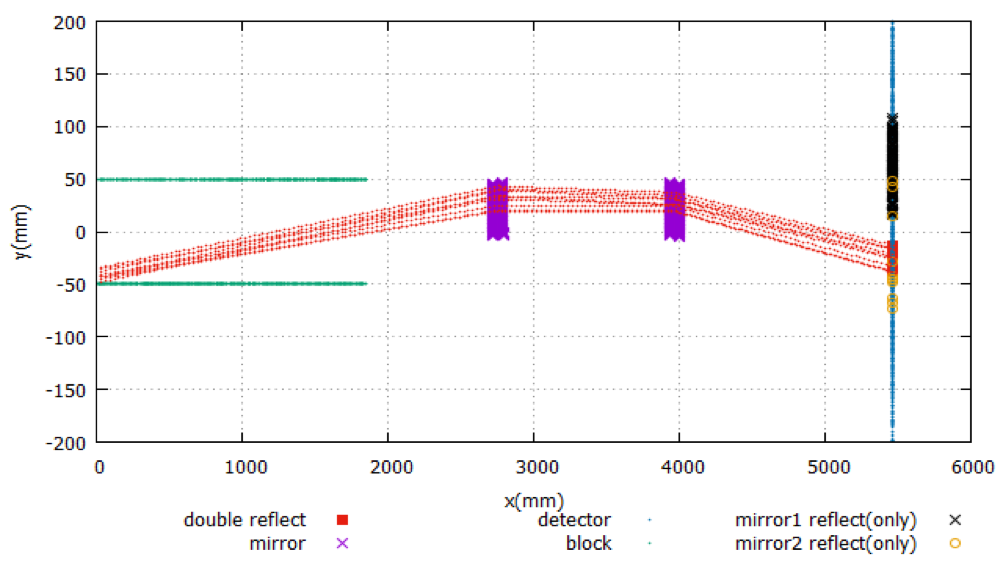
\includegraphics[keepaspectratio,scale=0.4]{angle/simulation.png}
\caption{シミュレーション例}
\end{figure}

これは装置を上から見た図であり、横軸xは粒子の進行方向、縦軸yは粒子の進行方向と垂直な方向を示す。粒子は$x=0$、$y=-50 \sim y=50$の間から角度は一様、エネルギーは予備実験で測定したKUANSのエネルギー分布に従って射出され、 検出器のある場所に到達する。ただし、途中で遮蔽ブロック、あるいはアナライザーに塗ってあるガドリニウムに衝突した場合はその時点で粒子は止まるものとしている。色は、紫はミラーのある位置を意味し、緑はブロックで止まった粒子を表している。また、赤が今回欲しい2回反射した粒子を表しており、他の色の粒子(水色はミラーに反射されなかった中性子、黒はポラライザーでしか反射されなかった中性子、黄色はアナライザーでしか反射されなかった中性子)と区別せねばならない。今回の図は2回反射された中性子を分かりやすくし、どの軌道を主に通るか分かるように軌道を赤色で示してある。

\subsection{コリメータによるビーム角度の最適化}

まず、ポラライザーのみを置いたシミュレーション結果が以下の通りである。(今回はポラライザーで反射した中性子を黒の軌道で表している。)

\begin{figure}[H]
\centering
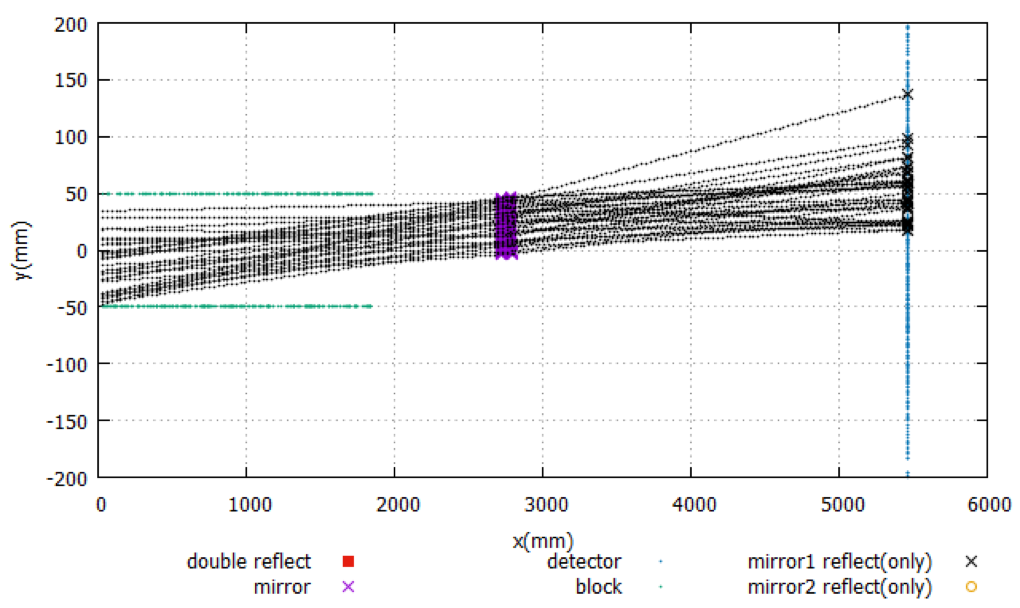
\includegraphics[keepaspectratio,scale=0.4]{angle/nocolimator.png}
\caption{コリメーションをしていない場合}
\end{figure}

今回分離しなければならないのはポラライザーで反射していない水色と、反射した黒を分離することである。しかし、この図でわかるように今の場合分離できておらず重なってしまっている。従って、この2つを分離する操作をする必要がある。今回分離できていない原因の1つとして、ビームが広がり過ぎてしまっていることが挙げられる。そのため、まずコリメーター部分でビーム幅を制限する事を考える。

まず、どの程度ビームを制限するかについてであるが、本実験で使用する$^3$He検出器は大きさが約$20$ mmであり、それ以上のビーム幅を持たせてもあまり意味がない。従って、今回はビーム幅を$20$mmで制限する。また、この$20$mmの幅のビームを$y=-50 \sim y=50$のどこから取り出すかであるが、予備実験の結果からビームは右側から多く射出されることが分かっているので、右側からビームを取り出す。そのため、ビームに$1.46$度の角度をつける。

以上の考察をもとにビームのコリメートをする。今回はビームを制限するためにビームの通過しない箇所をポリエチレンブロックで遮蔽する。その結果が以下の通りである。

\begin{figure}[H]
\centering
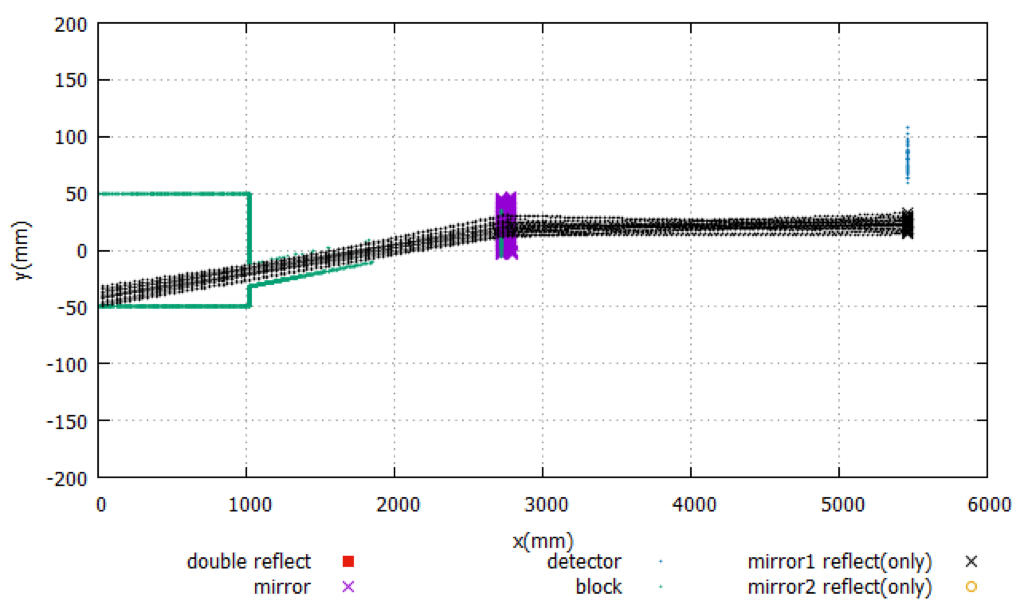
\includegraphics[keepaspectratio,scale=0.4]{angle/colimator.png}
\caption{コリメーションをした場合}
\end{figure}

図から分かるようにビーム幅を制限することによりポラライザーで反射した成分(黒)、反射しなかった成分(水色)を分離する事が出来た。

\subsection{ポラライザー角度の最適化}

次にミラー角度について考察をする。ミラーで反射した中性子と反射していない中性子を分けるにはミラーをビームに対して傾ければ良い。なぜなら、反射せず透過した中性子の軌道はミラーを傾けても変化しない一方、反射した中性子はより大きな角度をつけられて反射するからである。しかし、ミラーをビームに対して傾けすぎると相対角度が1度を超えてしまうため反射しなくなる。したがって、最も適切なミラーの角度を決める必要がある。また、中性子がガイド磁場の中心を通る必要があるため、中性子ビームとガイド磁場コイルとの平行度が高くなるよう考慮した。さらにその中で、反射される中性子が最も多くなるようにした。今回、ポラライザーの角度として$0.87$度、$0.67$度、$0.62$度で実験を行い結果を比較した。シミュレーション結果、PRMTによる実験結果は以下の通りである。ただし、RPMTによる結果はミラーによる反射成分を見やすいように波長3 Å以上の中性子のみに制限している。

\begin{figure}[H]
\begin{minipage}{0.50\hsize}
\begin{center}
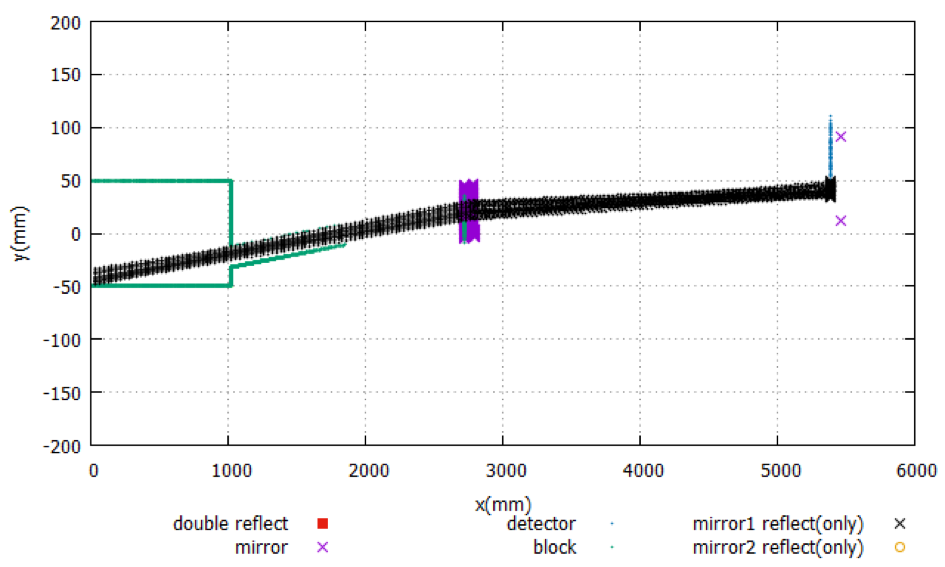
\includegraphics[height=4.5cm]{angle/polonesim.png}
\subcaption{0.87度のシミュレーション}
\end{center}
\end{minipage}
\begin{minipage}{0.50\hsize}
\begin{center}
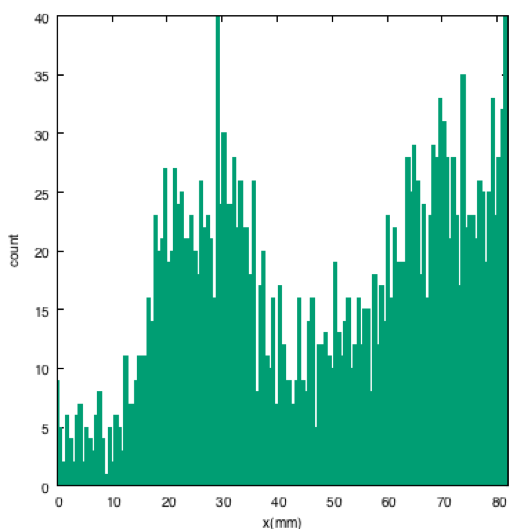
\includegraphics[height=4.5cm]{angle/poloneex.png}
\subcaption{0.87度の実験結果}
\end{center}
\end{minipage}
\caption{0.87度}
\end{figure}

\begin{figure}[H]
\begin{minipage}{0.50\hsize}
\begin{center}
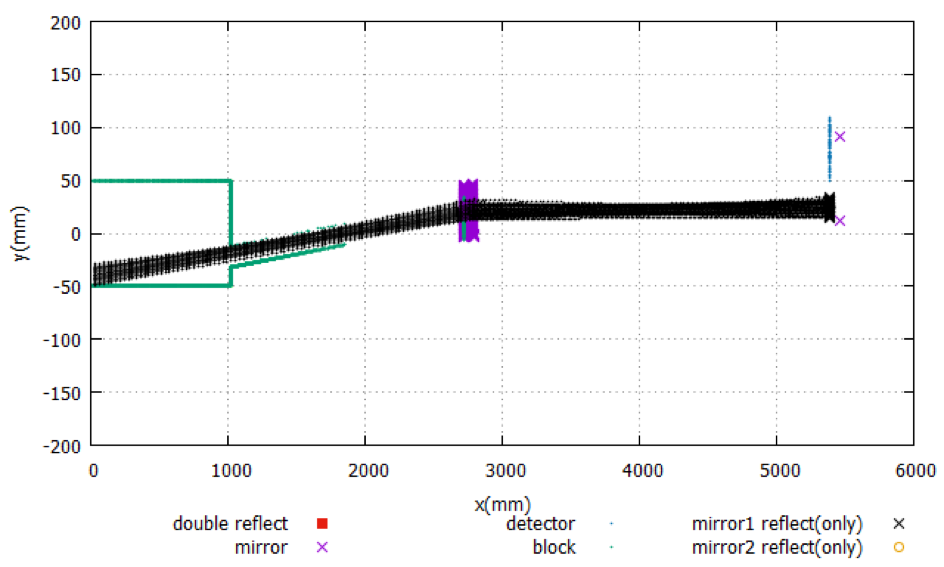
\includegraphics[height=4.5cm]{angle/poltwosim.png}
\subcaption{0.67度のシミュレーション}
\end{center}
\end{minipage}
\begin{minipage}{0.50\hsize}
\begin{center}
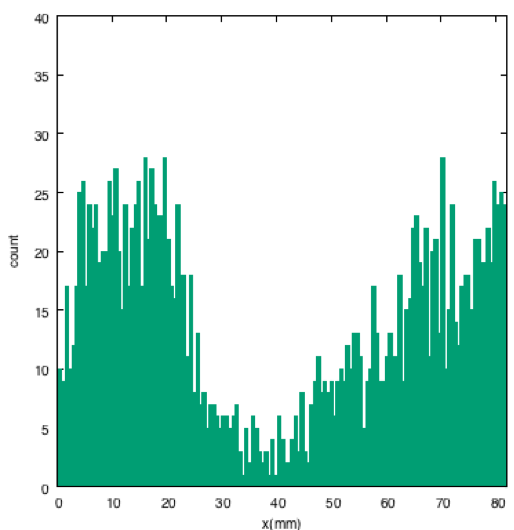
\includegraphics[height=4.5cm]{angle/poltwoex.png}
\subcaption{0.67度の実験結果}
\end{center}
\end{minipage}
\caption{0.67度}
\end{figure}

\begin{figure}[H]
\begin{minipage}{0.50\hsize}
\begin{center}
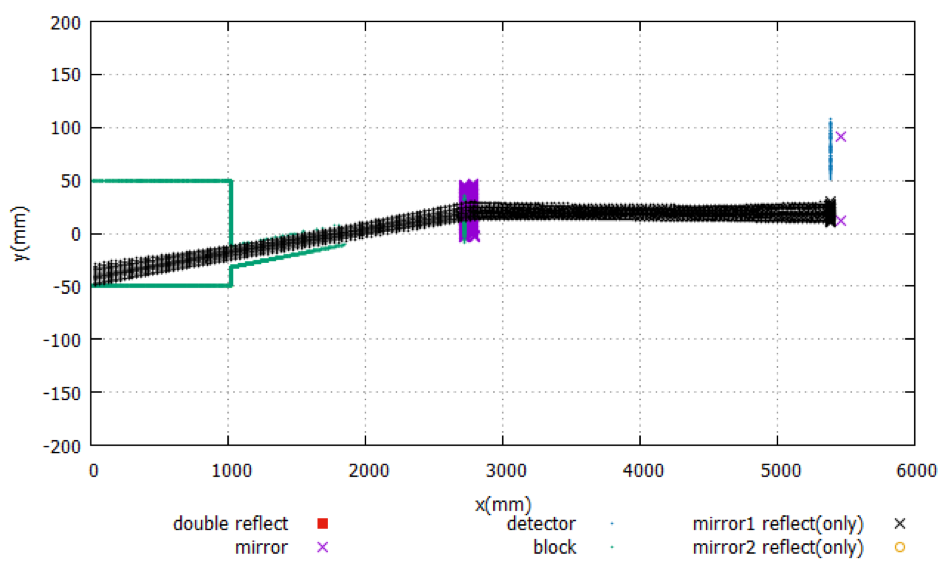
\includegraphics[height=4.5cm]{angle/polthreesim.png}
\subcaption{0.62度のシミュレーション}
\end{center}
\end{minipage}
\begin{minipage}{0.50\hsize}
\begin{center}
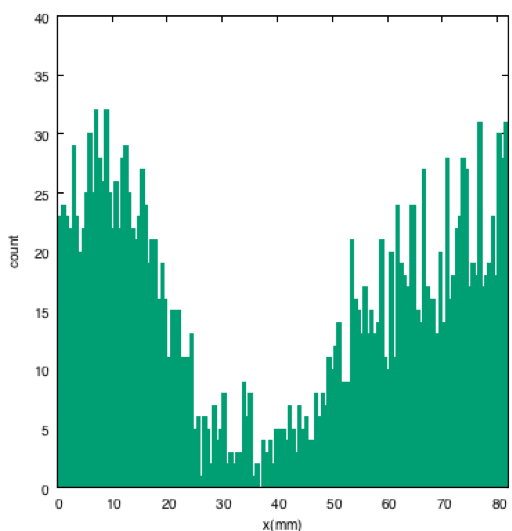
\includegraphics[height=4.5cm]{angle/polthreeex.png}
\subcaption{0.62度の実験結果}
\end{center}
\end{minipage}
\caption{0.62度}
\end{figure}

以上の結果を見ると、ミラーを平行にするほどビームは分離し、どの角度においてもビームが分離できている事がわかる。しかし、$0.87$度では重なってしまっている部分が存在する。また、$0.62$度ではビームがガイド磁場コイルに対して少し傾いてしまっている。したがって、今回はビームが綺麗に分離できており、かつビームがガイド磁場コイルに平行であるという理由からポラライザーの角度を$0.67$度に設定した。

\subsection{アナライザー角度の最適化}

アナライザー角度の設定については、ガイド磁場コイルとの平行度はすでに達成されているので、ミラーに一回反射した中性子と二回反射した中性子の分離、反射される中性子の数の増加の二点を満たすようにアナライザーの角度を設定した。アナライザー角度の設定についてもポラライザー角度の設定と同様に行い、ミラーの角度を$1.03$度に設定した。その結果が以下の通りである。

\begin{figure}[H]
\begin{minipage}{0.50\hsize}
\begin{center}
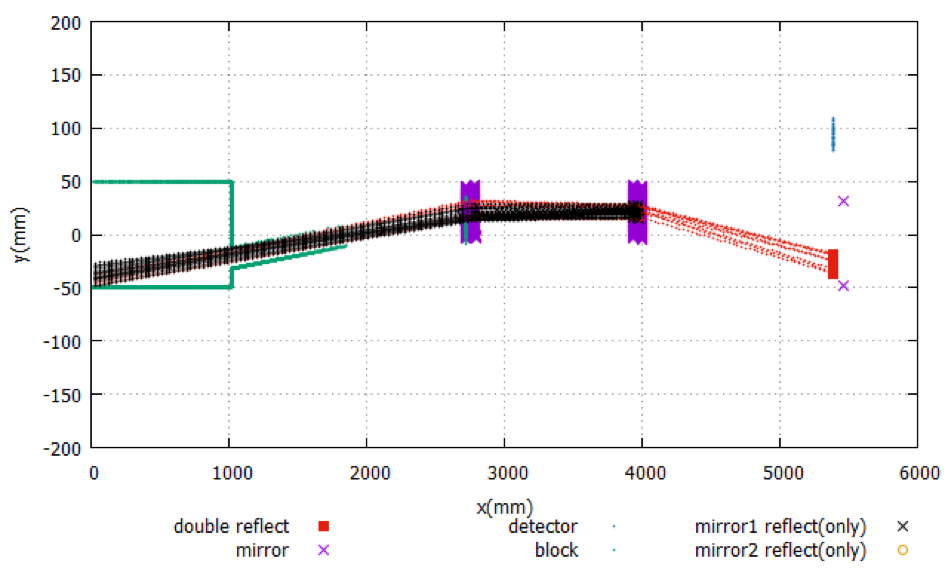
\includegraphics[height=4.5cm]{angle/anaonesim.png}
\subcaption{1.03度のシミュレーション}
\end{center}
\end{minipage}
\begin{minipage}{0.50\hsize}
\begin{center}
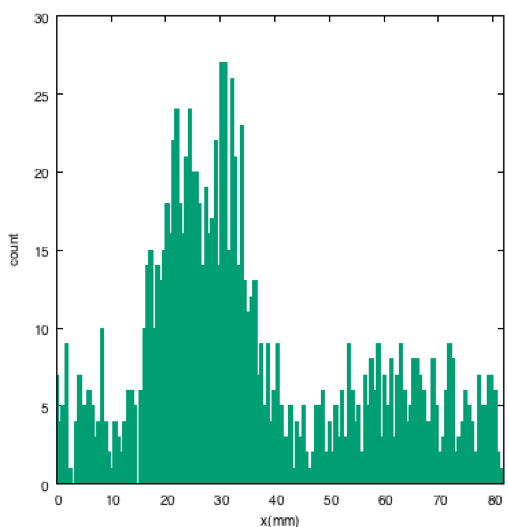
\includegraphics[height=4.5cm]{angle/anaoneex.png}
\subcaption{1.03度の実験結果}
\end{center}
\end{minipage}
\caption{1.03度}
\end{figure}

以上の結果より、ミラーで2回反射された中性子と、その他の中性子を分離する事ができた。
